\chapter{Methodology}
To ensure the success of this project a basic plan of action was created. The following diagram shows the critical phases of the project.

\begin{figure}[!ht] 
\captionsetup{width=0.8\linewidth, font=small}  
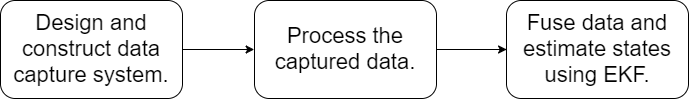
\includegraphics[width=0.8\linewidth]{figures/planOfAction.png}
  \caption{Diagram showing the progression and dependence of the major stages of this project}
\label{fig:planOfAction}
\end{figure}

Due to the availability of equipment, financial limitations and time constraints various design parameters where predetermined. These known design elements are discussed in the following section.
  
\section{System Design}
This section is dedicated to defining and understanding the specifications of the data capture system. The system will consist of 4 cameras and an IMU mounted to the torso of the subject. The cameras will record the lower limbs of the subject while the IMU will log inertial data from the body of the subject. The video data from the cameras will provide information about the kinematics of the lower limbs with respect to the cameras while the IMU will provide motion data of the body with respect to the inertial frame. As discussed in the previous chapter the inertial frame and the world frame are equivalent in this project. 

Due to the availability of equipment provided by the Mechatronics Lab the following equipment was chosen as the main components to use in the system:


\begin{table}[!ht]
\label{equipment-table}
\begin{tabular}{llll}
Item		 & Selected Equipment				& From		  			\\
Camera      & 4 GoPro Hero Session Cameras  & \cite{gopro} 		\\
IMU         & 1 Sony Xperia Z3 Compact      & \cite{sony}  		\\
Chest Mount & 1 Action Mount Chest Mount    & \cite{actionmounts}   
\end{tabular}
\caption{Known design elements of the project}
\end{table}

The specifications of this data capture system has been defined as:
\begin{itemize}
\item 2 stereo housings to hold the cameras
\item Chest mount to hold the cameras and IMU
\item Connecting hardware to mount camera housing to the chest harness.
\item Cameras must be stable during running
\item IMU must be rigidly mounted to front cameras
\item Cameras must capture full lower limb motion
\item Harness must be comfortable during running.
\item Harness must not impede natural gait of subject
\item Harness must be as light as possible
\item Harness must fit different size torsos and for different sexes
\item system must be remote controlled as far as possible 
\end{itemize}

These specifications ensure a system that can be used by a large demographic of people.

\section{Modelling the Lower Limbs}
To interpret the data and the underlying mathematics a model of the human torso and lower limbs must be created. This model consist of the lower limbs being represented as rigid links. Each leg is comprised of three different links: thigh, calf and foot. The joints connecting the links have been limited degrees of freedom to simplify the model. The ankle (serving as the joint between the foot and calf) is assumed to have a single rotational degree of freedom (pitch). The knee (serving as a joint between the calf and the thigh) has also been limited to only have a pitch element. Finally the hip (joining the thigh to the body) has been given 2 rotational degrees of freedom: pitch and yaw. This rigid model can be seen in the following figure.

\begin{figure}[!ht] 
\captionsetup{width=0.8\linewidth, font=small}  
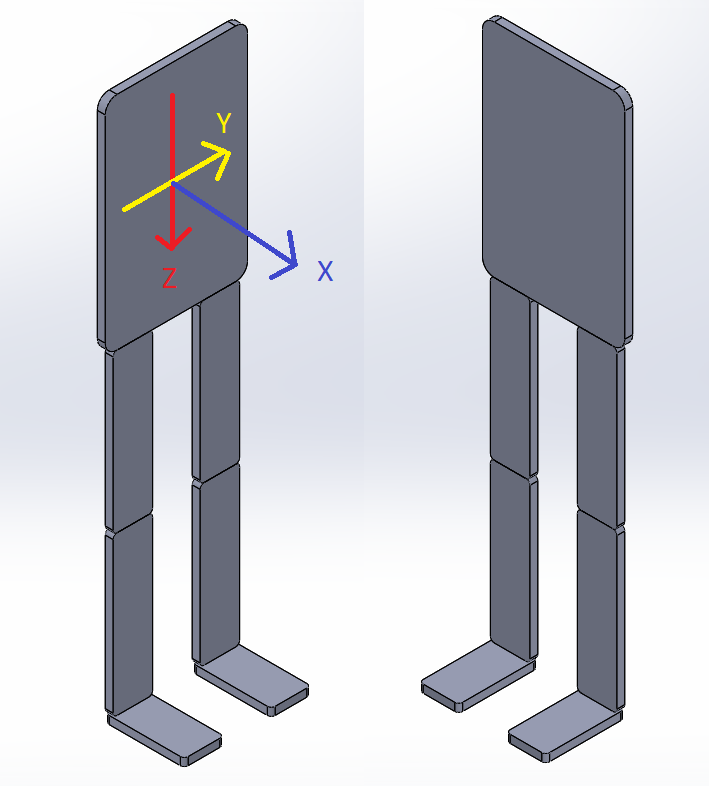
\includegraphics[width=0.8\linewidth]{figures/swmodel.png}
\caption{Rigid beam model used in this thesis}
\label{fig:swmodel}
\end{figure}




\section{Experimental Details}
The data was captured during a short straight road run where the runner started from a standing position and accelerated to a steady state run

\section{Sensor Fusion}


\section{Limitations}
The scope of this research does not include runs over rough terrain as this is the logical next step after flat ground steady state running is modelled and estimated. It is assumed that given robust EKF and complete image processing solution the system would work for running on various terrains.

Another source of limitations is the nature of the rigid beam model. This non elastic model does not take in to account the slight change in lengths of the limbs during running. The model also omits yaw and roll parameters about the knee and ankle as well as roll parameters about the hip. Finally the model assumes a rigid stationary chest that introduces some error relating the the camera data.

Since the chest swings proportional to the gait period this could be modelled as a harmonic oscillator. It would also be possible to interpret the rotational rates of the chest from the IMU data.







 



















